\chapter{Modelos Propuestos} \label{Chapter:5}

Tal y como se ha comentado en la \autoref{Chapter:TransferLearning}, la explotación de las técnicas de transferencia de aprendizaje y por lo tanto el empleo de unos modelos con una serie de pesos ya definidos con respecto a un conjunto de datos determinado, constituyen la base de los sistemas propuestos en este capítulo.

\begin{figure}
    \centering
    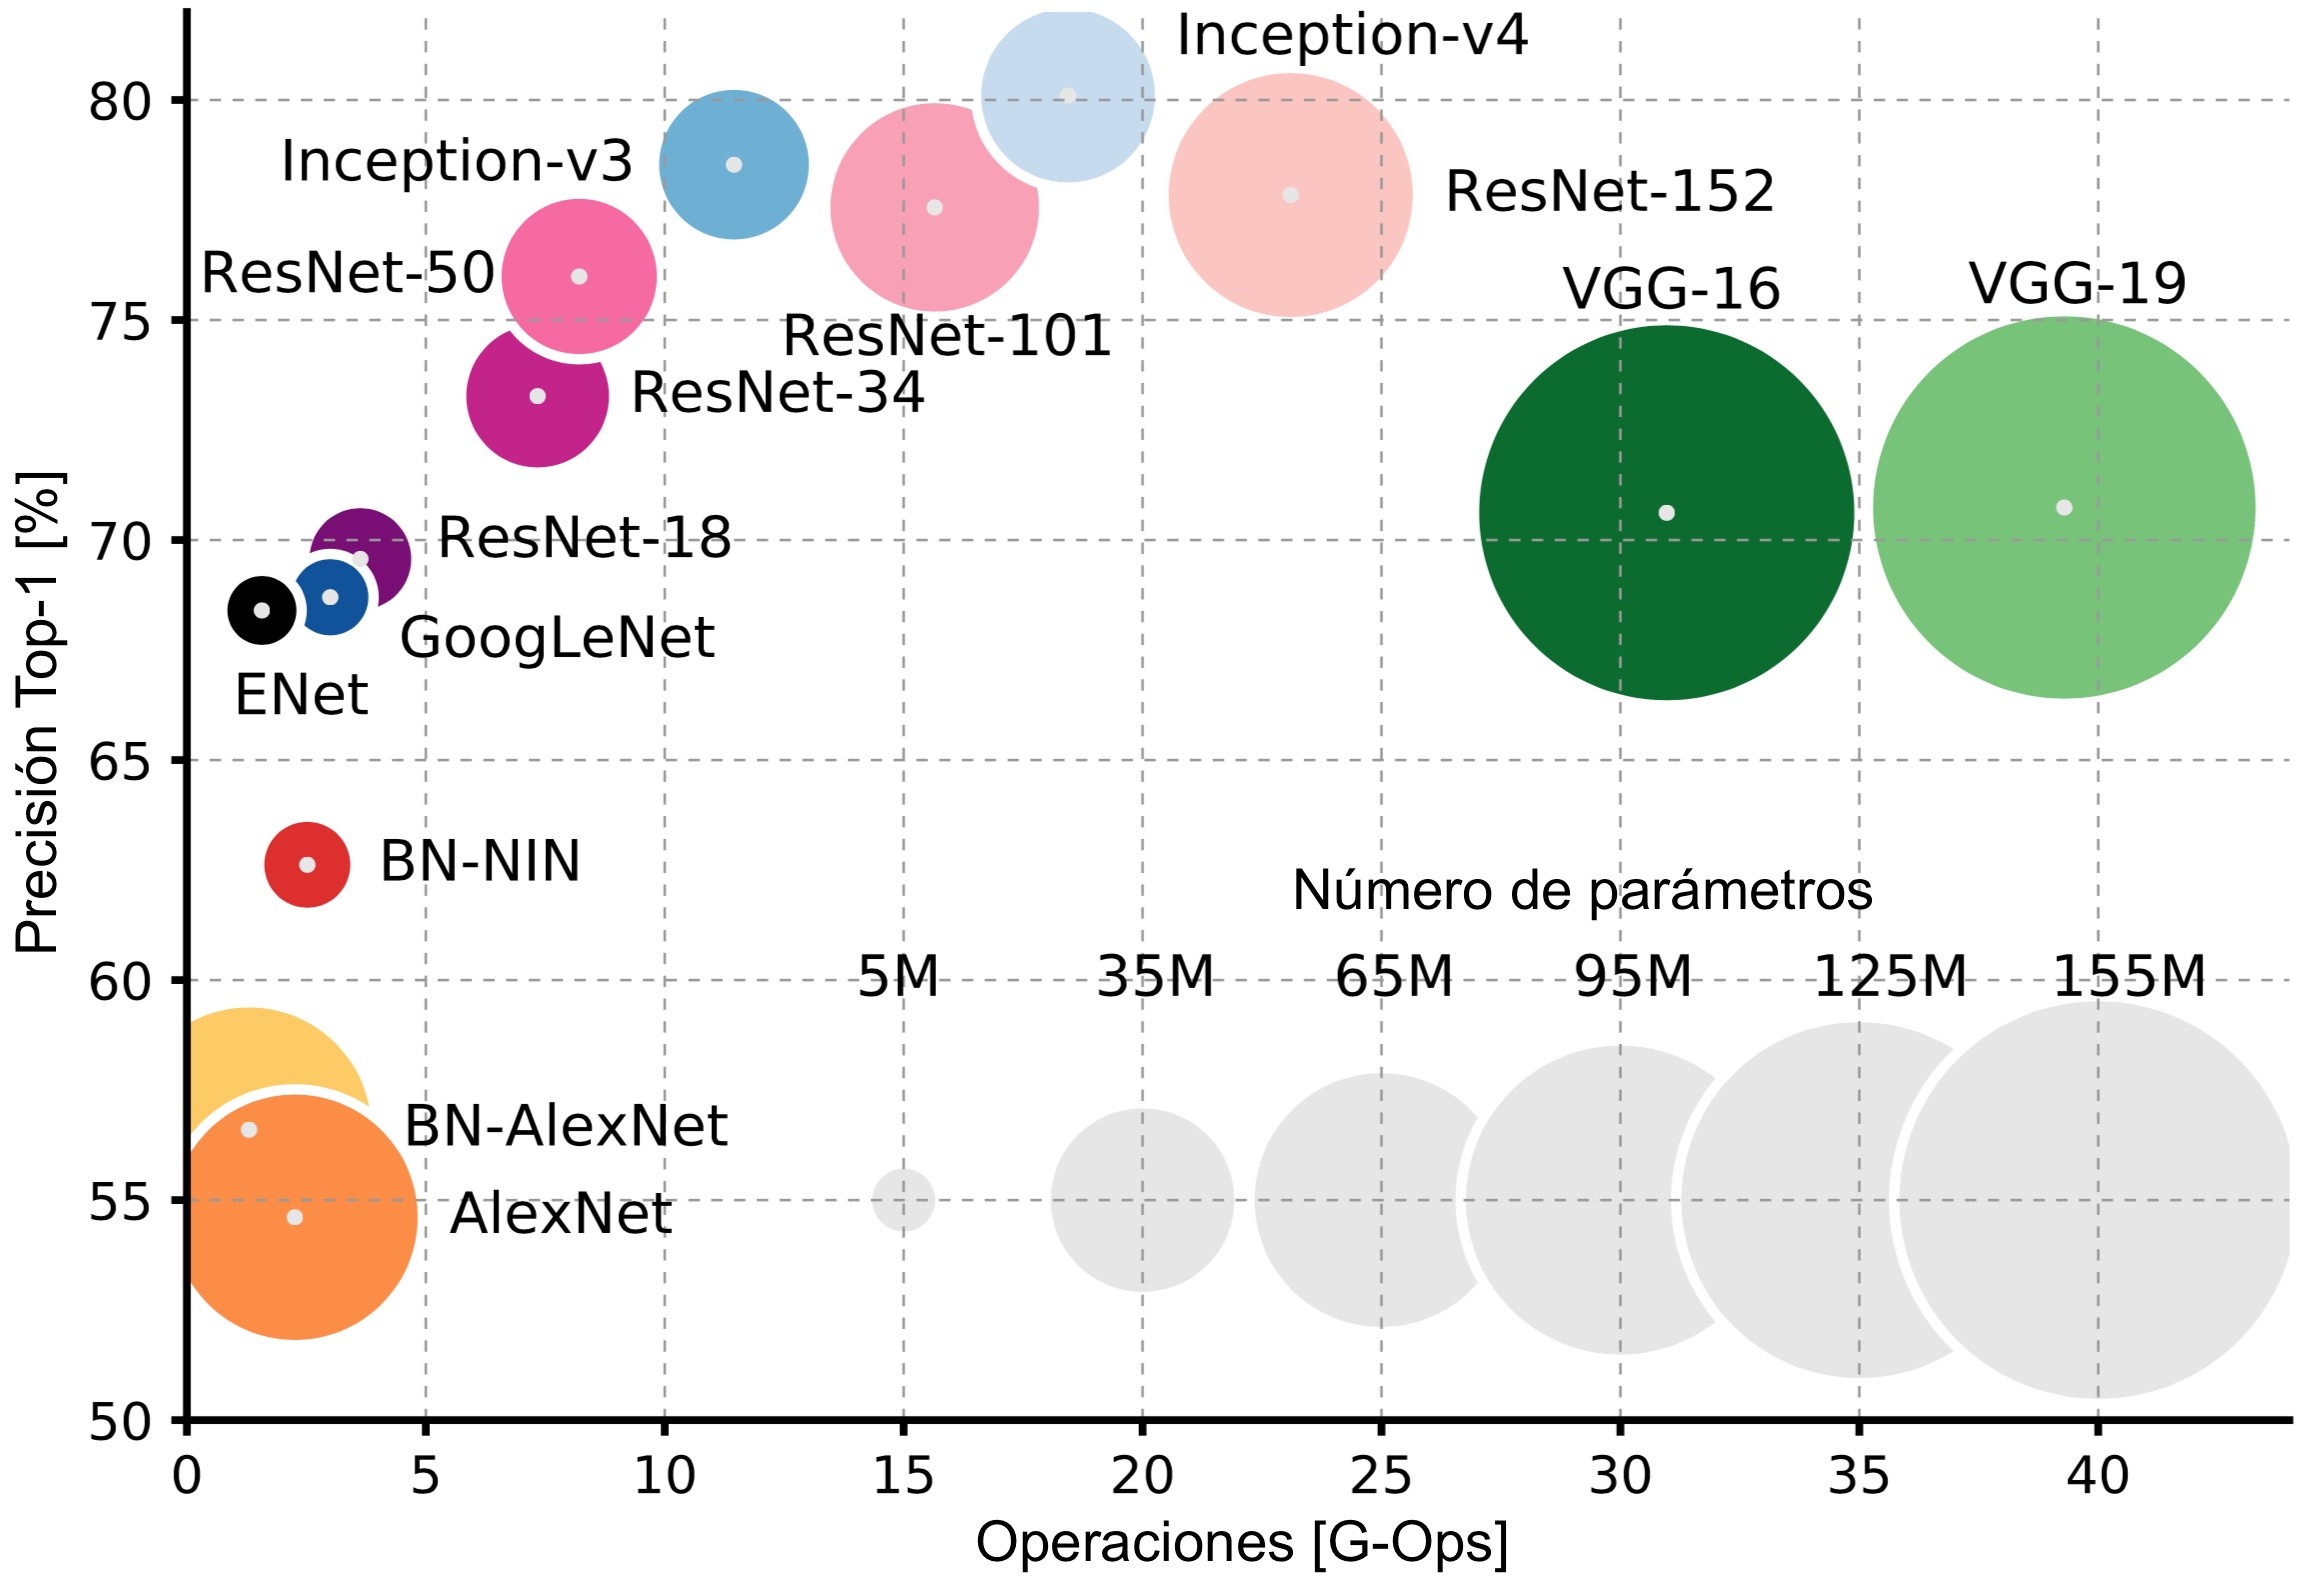
\includegraphics[scale=0.25]{Images/Models.png}
    \caption{Precisión Top-1 frente al coste computacional de una iteración del proceso de aprendizaje y el número de parámetros de la red \cite{Models}. Cabe destacar que aunque el modelo Inception-ResNet-v2 no se incluya en la figura, presenta características muy similares a Inception-v4 \cite{Inception-ResNet}.}
    \label{fig:Models}
\end{figure}

Por consiguiente, son utilizados en primera instancia los modelos Inception-v3 \cite{Inception-v3} e Inception-ResNet-v2 \cite{Inception-ResNet} con los pesos entrenados previamente sobre el conjunto de datos ImageNet descrito en la \autoref{Chapter:ImageNet}. Sin embargo, dado que las propiedades de las imágenes de esta base de datos difieren en gran medida de las características faciales que se intentan aprender y reconocer, se ha optado por explorar el uso de modelos más sencillos pero enfocados al reconocimiento facial. Es por ello que en última instancia se emplea el modelo ResNet-50 preetrenado con la base de datos VGGFace2 expuesta en la \autoref{Chapter:VGGFace2}. La comparación de estos modelos en el desempeño del desafío ILSVRC puede observarse en la \autoref{fig:Models}. Esta representación, además, escenifica la principal razón de la elección de estos modelos concretos: son los que mejores tasas obtienen con respecto al coste computacional y al número de parámetros.

Por último, obtenidos unos resultados más que aceptables y eficientes en lo que respecta al tiempo de entrenamiento, se ha intentado dar un paso más allá con la intención de mejorar las tasas de acierto y la calidad de la base de datos inicial mediante la implementación de una Red Generativa Antagónica (GAN) que permita la producción artificial de imágenes y, por lo tanto, la eliminación del desequilibrio de la distribución de clases del conjunto FER-2013.

En definitiva, a lo largo del proceso de desarrollo de un sistema de reconocimiento de expresiones faciales válido, se han ido explorando numerosas arquitecturas (Inception-v3, Inception-ResNet-v2 y ResNet-50) y técnicas (aumento de datos) con el objetivo de ir obteniendo cada vez mejores resultados sobre la base de datos FER-2013. Asimismo, a fin de permitir una comparación justa con respecto a los resultados de la \autoref{Chapter:RelatedWork}, son utilizados los protocolos de uso estipulados inicialmente por este desafío y que establecen la división de esta base de datos en tres conjuntos diferentes: entrenamiento, validación y evaluación.

\section{Afinación del Modelo Inception-v3}

Inception-v3 ha sido el resultado de las investigaciones llevadas a cabo por el equipo de Google para conseguir un modelo con una arquitectura cada vez más profunda e inteligente y capaz de desenvolverse de forma eficiente, tanto computacionalmente como cualitativamente, en el desafío ILSVR.

Su diseño, motivado por los experimentos a gran escala llevados a cabo sobre distintas redes convolucionales, gira en torno a cuatro principios básicos \cite{Inception-v3}:
\begin{itemize}
  \item Evitar los cuellos de botella, de modo que los datos fluyan de forma uniforme a lo largo de la red.
  \item Aumentar el número de dimensiones a medida que la información avance por la red. Las redes, de esta forma, se entrenarán más rápido.
  \item Bajar la resolución de la entrada antes de una capa convolucional promueve un aprendizaje más rápido y no da lugar a pérdidas significativas de la ganancia de información.
  \item Equilibrar el ancho y la profundidad de la red aumenta el rendimiento de las redes neuronales.
\end{itemize}

\subsection{Arquitectura}


\subsection{Preprocesamiento de los datos de entrenamiento}


\subsection{Entrenamiento}

\subsection{Resultados}



\cite{Inception-v3}
%Additionally, this paper uses Average Pooling instead of Fully Connected layers at the topof the ConvNet, eliminating a large amount of parameters that do not seem to matter much.There are also several followup versions to the GoogLeNet, most recently Inception-v4.




\section{Afinación del Modelo Inception-ResNet-v2}

\cite{Inception-ResNet}

\subsection{Preprocesamiento de los datos}

\subsection{Arquitectura}

\subsection{Entrenamiento}

\subsection{Resultados}








\section{Afinación del Modelo ResNet-50}
\cite{ResNet}

\subsection{Preprocesamiento de los datos}

\subsection{Arquitectura}

\subsection{Entrenamiento}

\subsection{Resultados}




\section{CycleGAN - Extensión de la Base de Datos FER-2013}

\subsection{Preprocesamiento de los datos}

\subsection{Arquitectura}

\subsection{Entrenamiento}

\subsection{Resultados}